It is time to put the attention on our (classical) daily lives. Arguably, the highlight of this century is \textit{data} (classical, at least for the first two decades), and motivating this Section by writing that \textit{we are surrounded by data} is, by now, a cliché, though an useful one. In turn, we are constantly faced towards new information and we ussually need to take decisions based on it (either conciously or unconciously)\footnote{The number of such decisions is obviously a random variable, but neuro-science community estimate it to be around 35K per day~\cite{sahakian_bad_2013}}.

While many of our daily decisions turns to be hard to model, some others can be placed on the scientific stage (\textit{i.e.} an experiment, where we acquire data in a systematic way). In this situation, we can riguoursly study the model and increase the possibilities of taking correct decisions in the face of uncertainty. In this context, we will now turn study (binary) hypothesis discrimination in Sec~\ref{ssec:1_hypo_testing}, and parameter estimation in Sec.~\ref{ssec:1_stinf_estimation}.

\subsection{Hypothesis testing}\label{ssec:1_hypo_testing}
The canonical example to discuss hypothesis testing problems deals with medical trials, where the effectiveness of a new development (for instance, a new test that tells whether a person has COVID or not) is to be tested. We will restrict to two hypothesis, or models, consisting on the null hypothesis $H_0$ (the patient is healthy), and the alternate hypothesis $H_1$ (the patient has COVID). In this context, we are interested in minimizing the chances that a sick patient is said to be healthy\footnote{By the 2020s, there was pandemics, and before having vaccines, we were particularly cautious when testing negative for COVID. For instance, we used to do double checks: if someone contracted COVID chances were extremely high to spread it among people in close contact with.}. This notion is captured by the overall probability that the test retrieves a \textit{false negative}, and is known as the $\beta$-error or type-II error. Denoting by $\hat{H}_i$ the result of the test, \textit{i.e.} $\hat{H}_1$ implies that the test result is \textit{positive} (diagnosing the patient as sick) and $\hat{H}_0$ \textit{negative} (telling the patient is healthy), have
\begin{align}
\beta = p(\hat{H}_0|H_1).
\end{align}
It is easy to come up with a test makes this quantity zero: always diagnose the patient as sick irrespective of the result obtained in the test. Such test is obviously useless, and we are often interested in keeping the \textit{false positive} rate bounded. This quantity is given by the $\alpha$-error, or type-II error:
\begin{align}
\alpha = p(\hat{H}_1|H_0).
\end{align}
We refer to $\alpha$ and $\beta$ as \textit{weak} errors, since they certify the average performance of the test; on the contrary, when discussing sequential strtegies we will also deal with the notion of \textit{strong certification}, in the sense that we will be interested in prodiving guarantees for \textit{each} realisation of the stochastic proceses.

In general it is not possible to minimize both errors and a tradeoff appears: reducing one type of error typically increases the other. Conventionally, we are interested in minimizing $\beta$ for a fixed value of $\alpha$, and this is known as \textit{assymetric hypothesis testing}. On the contrary, there are situations where both type of errors need to be minimized, and thus we consider a linear combination of the errors, leading to the \textit{symmetric} error probability. In particular, the total or mean error probability is given by
\begin{equation}\label{eq:1_statinf_symm}
P_e =  p_0 p(\hat{H}_1|H_0) + p_1 p(\hat{H}_0|H_1),
\end{equation}
where $p_k$ stands for the prior probability of having the $k^{\text{\underline{th}}}$ model (and $k=0,1$), and $\sum_k p_k=1$. Analogously, the success probability is defined as
\begin{equation}\label{eq:1_statinf_symm_ps}
P_s= 1-P_e =  p_0 p(\hat{H}_0|H_0) + p_1 p(\hat{H}_1|H_1),
\end{equation}
Our notation emphasizes that the symmetric error can be interpreted Bayesianly, where prior probabilities are assigned to each hypothesis and the total error is obtained by multiplying each prior with the postirior probability of having such hypothesis given the observed data.

Let us consider the example of a discrete random variable $X$ (say a dice) which takes values $x\in\{0,1,\ldots n\}$, with probability distribution $p(x)$ under hypothesis $H_{0}$ or $q(x)$ under hypothesis $H_{1}$. Upon receiving a sample, i.e. a value $x$, we have to make a guess $\hat{H}_{g(x)}$ about the true hypothesis according to a \emph{decision or guessing rule} $g(x)\in\{0,1\}$. The total success probability can be written as
\begin{align}
P_{s}&= \sum_{x=1}^{n} \left(P(g(x)=0,x|H_{0})\pi_{0}+P(g(x)=1,x|H_{1})\pi_{1} \right)\nonumber\\
&\leq \sum_{x=1}^{n} \max\{P(g(x)=0,x|H_{0})\pi_{0},P(g(x)=1,x|H_{1})\pi_{1}\}
\end{align}

This upper bound can be attained by always guessing for the most likely hypothesis: i.e.
\begin{equation}
g(x)=\left\{\begin{array}{ll}
0 & \mbox{ if } P(x|H_{0})\pi_{0}\geq P(x|H_{1})\pi_{1} \\
1 &\mbox{ if } P(x|H_{0})\pi_{0}\leq P(x|H_{1})\pi_{1})
\end{array}\right.
\end{equation}
That is the \textit{maximum-likelihood} criterium is optimal for the minimum-error case (symmetric error probability optimization).

Before further discussing hypothesis testing and the assymetric scenario, we will discuss a situation in which the underlying models are quantum states. That is, given a copy of a quantum state we are asked to correctly label it. However, this situation is subtle: the maximum-likelihood criterium can only be applied once a particular measurement (POVM) is implemented, and this is of course also subject to optimization.
\subsection{Single-shot quantum state discrimination}\label{ssec:1_qdisc}
Analogies and similarities do certainly allow us to build intuition, but we do also rely on differences to asses the \textit{meaning} of physical phenomena. We do not need to go very far: discriminating between these letters allows us to be reading this thesis. Suppose, on the other hand, that your glasses drop all of a sudden: you will definitely find difficulties to distinguish between letters. This means that some kind of \textit{noise} appears, and hinders ---at least partially--- the information to be perfectible discernable. At zero-noise level we are able, in principle, to perfectly tell which are the letters. Thus, in  classical scenarios, external noise-sources are the only cause for which letters might not be perfectly distinguishable.

However, in the quantum realm, letters might well be in a superposition. As such, we ussually encounter situations in which even at zero-noise level, not perfect distinguishability can be achieved when looking measuring the (quantum) information, a phenomena unrelated to the transmission channel, but intrinsically linked to the quantum nature of information.

While no glasses can help to achieve perfect distinguishability of quantum states, we are here interested in studying optimal ways to distinguish between the symbols, \textit{e.g.} given now by quantum states. As a matter of fact, among all the possibilities allowed by quantum mechanics to extract information out of a system, some measurements are more helpful than others when it comes to discriminate between a given set of quantum states. Moreover, quantum physics provides an ultimate limit to the distinguishability of states, a fact that we will now turn to discuss.

\subsubsection{The Helstrom bound}\label{sssec:hb}
We focus on the one-shot discrimination problem between two quantum states $\rho_0$ and $\rho_1$. Given a single copy of a state $\rho$, the task is to tell if either hypothesis $H_0: \rho = \rho_0$ holds, or hypothesis $H_1: \rho = \rho_1$ does it, each having a prior probability of ocurring $p_k$, with $\sum_k p_k = 1$. To this end, we introduce a two-outcome POVM $\mathcal{M} = \{ M_0, M_1\}$ such that $\sum_{k=0}^1 M_k = \mathbb{I}$ and $\mathcal{M}_k\geq0$.
Based on the measurement outcome $k$, the decision rule reads $\hat{k} = k$~\footnote{Note that we do not lose generality by restricting to two outcomes POVM, since any POVM with more outcomes, $\llaves{E_i}_{i=1}^n$ can be regrouped in an effective POVM with the same performance: $M_0 = \sum_{i\in S_0} E_i$, and $M_1 = \sum_{i\in S_1} E_i$ where $S_k$ is the set of outcomes for which we guess hypothesis $k$.}while the outcome probability is given by Eq.~\ref{eq:bornrule}, \textit{e.g.} $p(k|\rho) = \tr{M_k \rho}$. The success and error probabilities of such discrimination protocol is given by
\begin{align}\label{eq:1_qdisc_PSEMM}
P_s(\mathcal{M}) &= \sum_{k=0,1} p_k\; p(\hat{k}|k) =\sum_{k=0,1} p_k \;\tr{\rho_k M_k}, \\
P_e(\mathcal{M}) &=  \sum_{k=0,1} p_{\bar{k}} \; p(\hat{k}|\bar{k}) = \sum_{k=0,1} p_{\bar{k}} \;\tr{\rho_{\bar{k}}} M_k = 1-P_s(\mathcal{M}), \nonumber
\end{align}
where we define the complementary hypothesis $\bar{k} = k+1$ (modulus 2). Under these definitions, we will now derive a lower bound for the error probability, known as \textit{the Helstrom Bound}. To this end, let us write the error probabiliy as per
\begin{align}
P_e(\mathcal{M}) &= p_0 \tr{M_1\rho_0} + p_1 \tr{M_0\rho_1} \\
&= \tr{(\mathbb{I} - M) \tilde{\rho_0}} + \tr{M \tilde{\rho_1}} \nonumber
\end{align}
where we define $M=M_0$ and $\tilde{\rho_k} = p_k \rho_k$ as a shorthand. Moreover, we let $\Delta := \tilde{\rho_0} - \tilde{\rho_1}$, it follows that while $\tilde{\rho_k}$ is a positive semi-definite operator, $\Delta$ might not be so, although is Hermitian and thus admits a diagonal representation. Having this in mind, we define $\Delta_\pm$ as the positive and negative part of $\Delta$ respectively, each being a positive-define operator, \textit{i.e.}
\begin{align}
\Delta_\pm &= \sum_{\lambda : \lambda\underset{<}{>0}} \lambda \ket{\lambda}\bra{\lambda}, \spacee \Delta= \Delta_+ - \Delta_-.
\end{align}
Then, we have that
\begin{align}
P_e(\mathcal{M}) = \tr{\tilde{\rho_0}} - \tr{M \Delta} &=\tr{\tilde{\rho_0}}  - \big(\tr{M \Delta_+} -\tr{M \Delta_-}\big)\\ \nonumber
&\geq\tr{\tilde{\rho_0}}  - \tr{M \Delta_+}\\ \nonumber
&\geq\tr{\tilde{\rho_0}}  - \tr{\Delta_+}\\ \nonumber
&= \tr{\tilde{\rho_0}} - \frac{1}{2}\Big(|| \Delta ||_1 + \tr{\Delta}\Big) \\ \nonumber &=  \frac{1}{2}\big( 1 - ||p_0 \rho_0 - p_1 \rho_1 ||_1),\nonumber
\end{align}
where we used that the operators $M$ and $\Delta_-$ are positive semi-definite, and that $\tr{\Delta_+} = \frac{1}{2}\Big(|| \Delta ||_1 + \tr{\Delta}\Big)$, which follows from the fact that  $|| \Delta ||_1 = \tr{|\Delta|} = \tr{\Delta_+} + \tr{\Delta_-}$.

The structure of the optimal POVM $\mathcal{M}^*$ can be obtained as follows. Assuming $\Delta$ has no vanishing eigenvalues, then $M = \Pi_+$, where $\Pi_+$ is the projector over the positive eigenspace $\Delta_+$, implying that $M_1 = \mathbb{I} - M_0$ projects onto the negative part of $\Delta$. For this case, the error probability reads
\begin{align}\label{eq:1_qdisc_helstom}
P_e(\mathcal{M}^*) &= \tr{\tilde{\rho_0}} - \tr{\Pi_+ \Delta} \\ \nonumber
&=\tr{\tilde{\rho_0}}  - \big(\tr{\Pi_+ \Delta_+} -\tr{\Pi_+ \Delta_-}\big)\\ \nonumber
&= \tr{\tilde{\rho_0}} - \frac{1}{2}\Big(|| \Delta ||_1 + \tr{\Delta}\Big) \\ \nonumber
&= \frac{1}{2}\big( 1 - ||p_0 \rho_0 - p_1 \rho_1 ||_1). \nonumber
\end{align}

While the optimizing measurement $\mathcal{M}^*$ is a projector, it a quite particular one, which requires access to the positive and negative subspace of $\Delta$. As such, obtaining its expression can be challenging, since it is not always possible to diagonalize $\Delta$. Moreover, we are often concerned with a physical implementation of that measurement, which is a subtle matter that will be discussed in Chapter~\ref{chapter:RLCOH}.

\subsubsection{The pure-states case}
As an example, let us consider the case of two arbitrary pure states $\ket{\psi}$ and $\ket{\phi}$. Here, the operator $\Delta$ can be written in a two-dimensional basis spanned by $\ket{\psi}$ and its orthogonal complement $\ket{{\psi}^\perp}$, and the Helstrom bound reduces to:
\begin{align}\label{eq:helstrom_pure}
P_e(\mathcal{M}^*, \ket{\psi_0}, \ket{\psi_1}) = \frac{1}{2}\Big(1 - \sqrt{1 - 4 p_0 p_1 |c|^2}\Big),
\end{align}
where $c = \langle \psi | \phi\rangle$ is the overlap between the pure states; as seen in Fig.~\ref{fig:helpure}, the bound tends to $\frac{1}{2}$ (\textit{i.e.} randomly guessing) as the overlap between the states approaches to unity, whereas it goes to zero when the states become orthogonal, which can be understood as a the classical limit. The optimal measurement is a projector onto a superposition of $\ket{\psi_0}$ and $\ket{\psi_0^\perp}$.

To see this, we can readily construct an orthogonal basis that spans the two-dimensional subspace of the Hilbert space needed to represent the states $\llaves{\ket{\psi}, \ket{\psi}}$. This can be done, for example, via Gram-Schmidt decomposition, where we consider
\equ{\ket{\psi^\perp} = \frac{\ket{\phi} - c \ket{\psi}}{\sqrt{1-|c|^2},}}
allowing us to write
\equ{\ket{\psi} = c \ket{\alpha} + s\ket{\alpha^\perp},}
where we defined $s=\sqrt{1-|c|^2}$. Now, the operator $\Delta$ can be represented in the two-dimensional space spanned by $\llaves{\ket{\alpha}, \ket{\alpha^\perp}}$ as per
\begin{align}
\Delta = \pi_0 \proj{\psi} - \pi_1 \proj{\phi} \equiv \Big(\begin{matrix}\pi_0 - \pi_1 c^2 &- \pi_1 c \;s \\-\pi_1 \bar{c}\;s&- \pi_1 s^2 \\\end{matrix}\Big).
\end{align}
An straightforward diagonalization leads to the eigenvalues of $\Delta$:
\equ{\lambda_\pm = \frac{1}{2}\Big(1 - 2 \pi_1 \pm \sqrt{ 1 + 4 \pi_0 \pi_1 |c|^2 }\Big),}
where we can readily see that expression in Eq.~\ref{eq:helstrom_pure} is obtained by inserting the trace-norm of $\Delta$ in Eq.~\ref{eq:1_qdisc_helstom}. Moreover, we can also compute the eigenstates (each associated to the positive and negative parts of $\Delta$) as per
\begin{align}\label{eq:projectors_pure}
\ket{\lambda_+} &= \alpha_1 \ket{\psi} + \alpha_2 \ket{\psi^\perp} \\
\ket{\lambda_-} &= \alpha_3 \ket{\psi} + \alpha_4 \ket{\psi^\perp},
\end{align}
where the coefficients are included in the footnote\footnote{\begin{align}\alpha_1 &=  -\frac{1}{2} \sqrt{2 \sqrt{1-c^2}+2} \\
\alpha_2 &= \frac{c}{\sqrt{2} \sqrt{\sqrt{1-c^2}+1}}\\
\alpha_3 &= \frac{c^2+\sqrt{1-c^2}-1}{\sqrt{2} \sqrt{\left(c^2-1\right) \left(\sqrt{1-c^2}-1\right)}}\\
\alpha_4 &= \frac{c}{\sqrt{2-2 \sqrt{1-c^2}}}\end{align}}. Recalling that the optimal POVM is constructed by projecting over $\ket{\lambda_\pm}$, we observe that generally the state we project over is a superposition between $\ket{\psi}$ and $\ket{\phi}$, \textit{e.g.} the hypothesis we aim to distinguish. This will play an important role when discussing the discrimination between two coherent states, since we can readily see that the optimal POVM in this case is a projection onto a cat-like state, \textit{e.g.} a superposition of coherent-states.

\begin{figure}[t!]
    \centering
    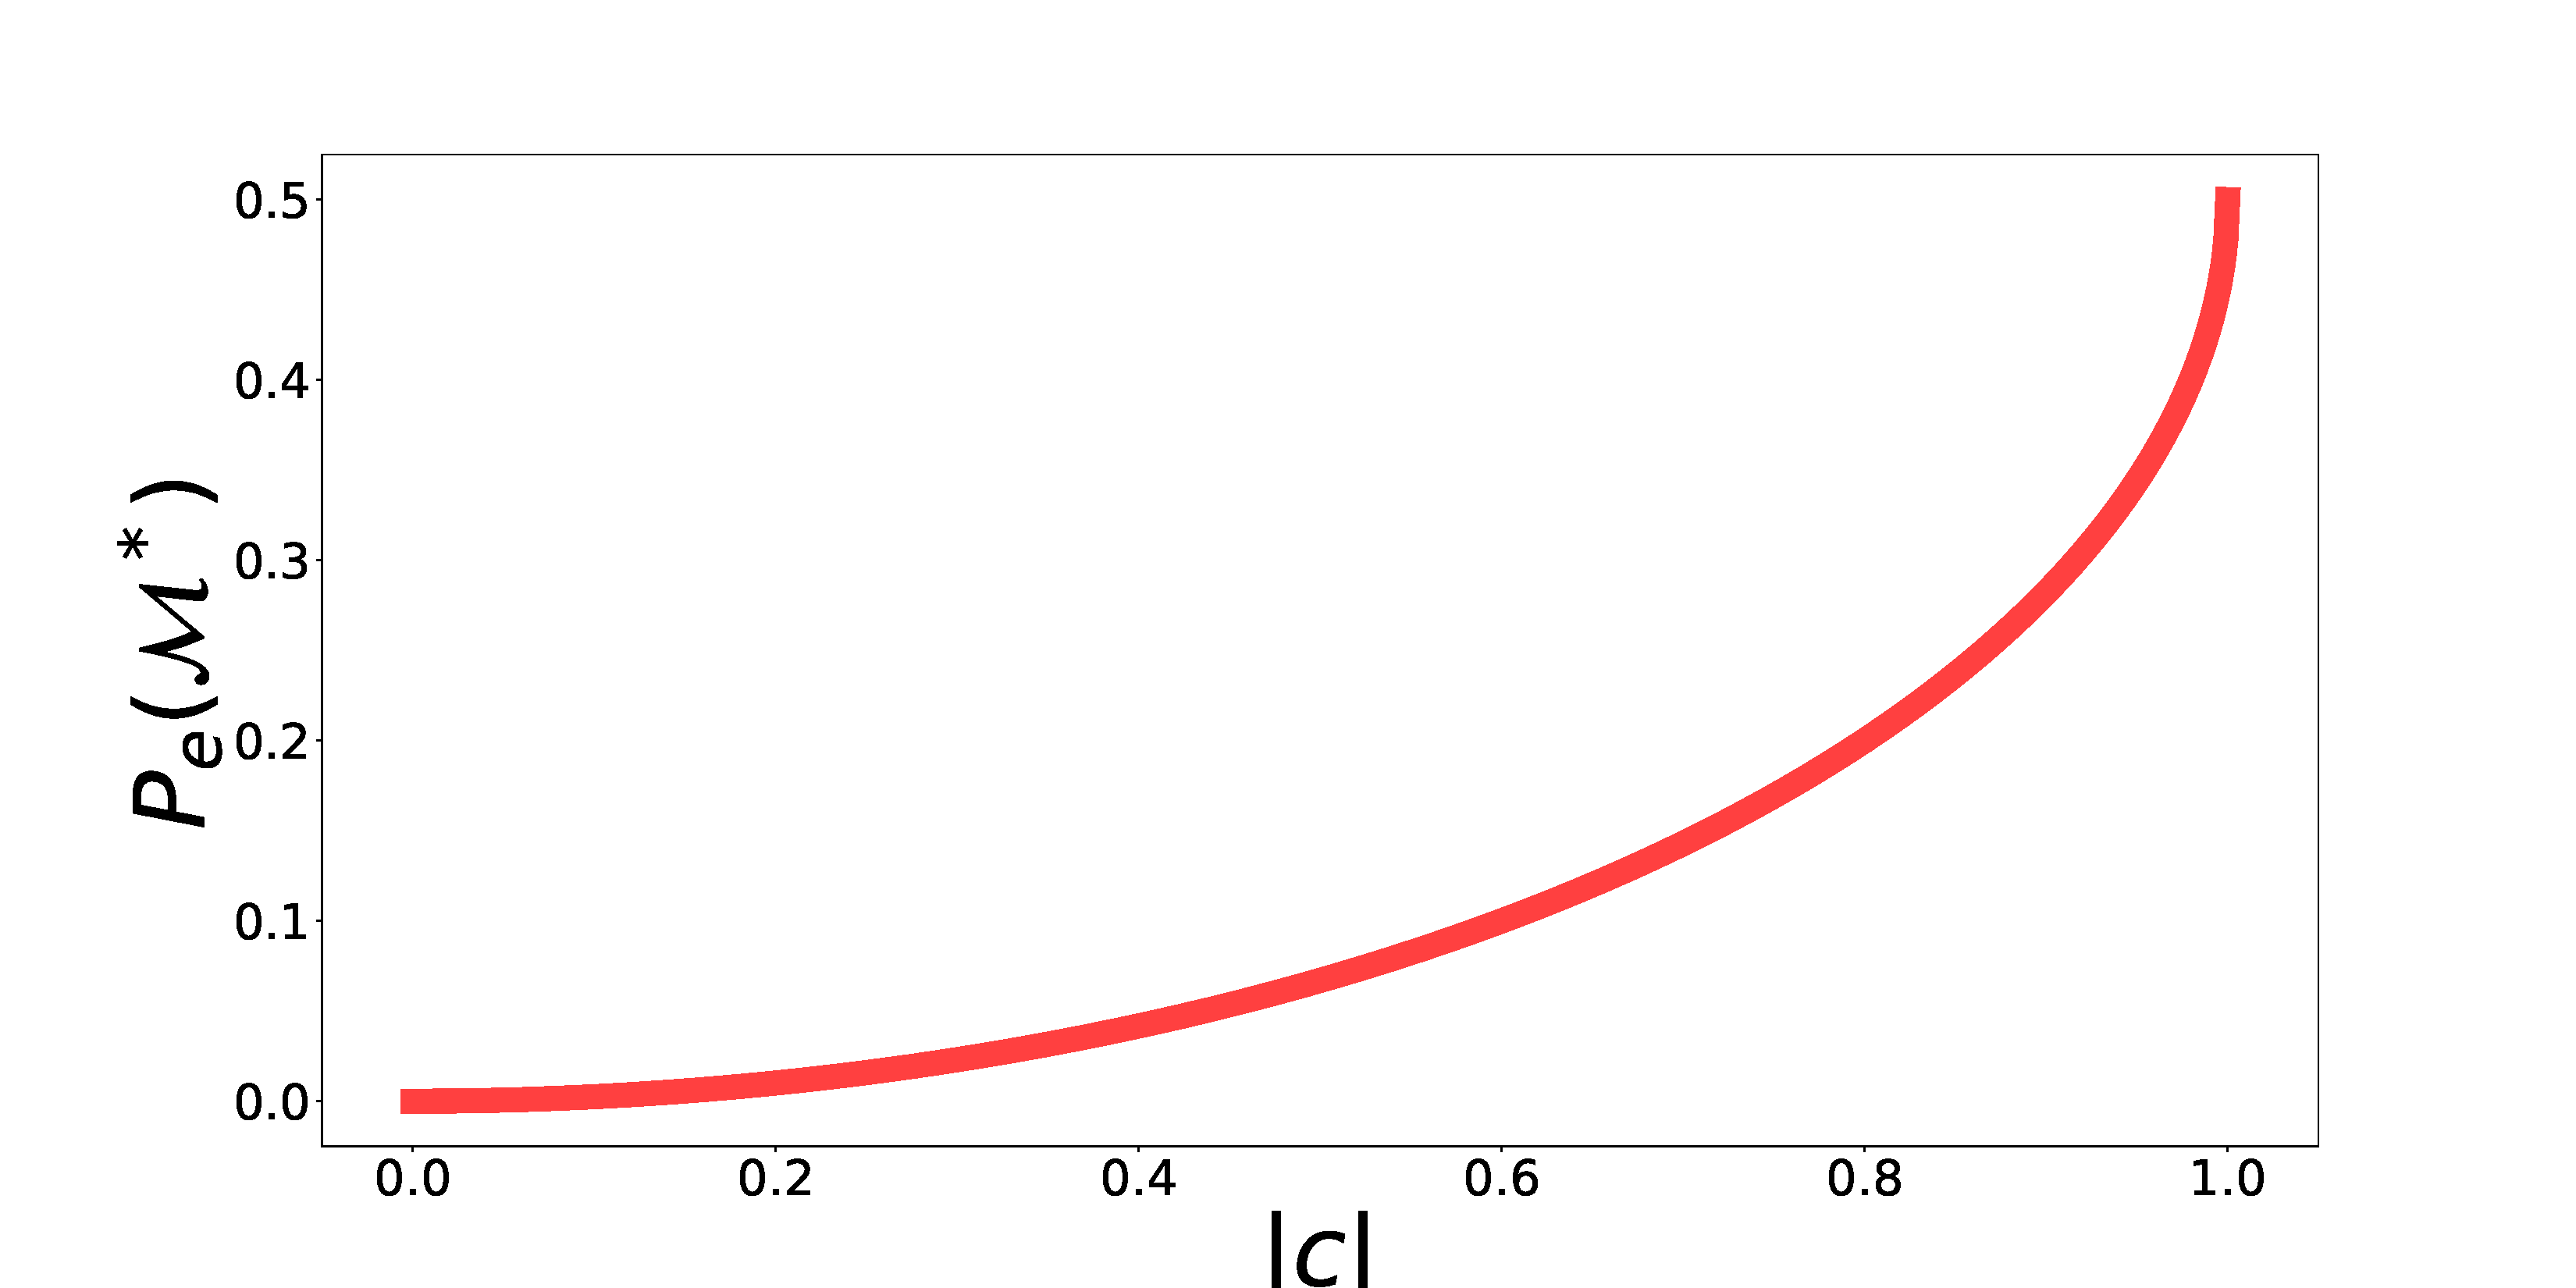
\includegraphics[width=1.\textwidth]{Figures/117/helstrom.pdf}
    \caption{We show Helstrom bound for the error probability when discriminating between two pure states as a function of their overlap $c$ (aboslute value).}
    \label{fig:helpure}
\end{figure}

To sum up, we have discussed the basics of single-shot quantum state discrimination; long is the road that continues this discussion. For instance, we ommited unambiguous state discrimination, where we demand that every time we guess for one hypothesis no errors are commited. This requires that we allow an extra \textit{I don't know outcome}, that deems that data inconclusive; in such case we are interested in minimizing the probability associated to such inconclusive outcome.

Also, we have not discussed multiple-hypothesis problems. In particular, closed-form solutions are known if the states are generated by a symmetry group; here, the optimal POVM is the \textit{pretty-good} (or square-root) measurement, and can be obtained explicitely in terms of the candidate states. In the non-symmetric case, such measurement often provides a \textit{pretty-good} success probability~\cite{Wooters1994prettygood, CrokeReviewQSD}. Also it is worth mentioning that semidefinite programming~\cite{boyd} will not be discussed here. The latter is a technique that allows to efficiently convex optimization problems (and relates to state discrimination when numerically optimizing over measurements).

%



% \subsubsection{Beyond minimum-error state discrimination}
% \textit{Unambiguous state discrimination} The POVM $\mathcal{M}$ can be constructed in such a way to allow for unambiguous discrimination, at the cost of potentially label outcomes as unconclusive. Here, $\mathcal{M} = \{ M_0, M_1, M_? \}$, and the unconclusive outcome is obtained with probability $p_?(\mathcal{M}) = \sum_{k=0,1} p_k p(?|k)$. For instance, in the case of pure states, we can readily construct the measurement operators as projectors onto orthogonal subpsaces of the states constituing the hypothesis; these are $M_0 = \frac{\proj{\psi_1^\perp}}{1+\braket{\psi_0}{\psi_1}}$ (guesses for $\ket{\psi_0}$),
% $M_1 = \frac{\proj{\psi_0^\perp}}{{1+\braket{\psi_0}{\psi_1}}}$
% (guesses for $\ket{\psi_1}$) and $M_? = \mathbb{I} - M_0 - M_1$ (leading to the unconclusive outcome); note that the accompanying coefficients of the projectors ensure that $M_? \geq 0$. We can readily see that when either outcome 0 or 1 are obtained, the test is conclusive, while a finite probability of unconcluding the test arises. In this setting, the challenge is thus to minimize the probability of undeciding, which is certainly relevant if no errors can be admitted in the discrimination task.
%
% \textit{Multiple-state discrimination $\&$ the Pretty Good Measurement}. We have seen that the optimal measurement in the minimum-error binary discirmination scenario is given by a complicated projection defined by the states to be distinguished. The optimal measurement in the multiple-hypothesis scenario has in general an unknown structure; nonetheless a \textit{pretty good measurement} (or square root measurement) can be derived, which in different scenarios such as symmetric pure states turns out to be optimal. Such approach constructs the optimal measurement from the square root of a mixture between the hypothesis states~\cite{Wooters1994prettygood, CrokeReviewQSD}.
%
% \textit{Semi-definite programming}. The optimization over POVM can be casted as a convex problem, which in turn can efficiently be solved through. Moreover, a dual problem can be formulated, which sometimes allows for analytical solutions (or bounds) useful for the problem at hand. For instance, it has been shown using this technique that the Dolinar-type receivers we consider in Chapter~\ref{chapter:RLCOH} can not be optimal when dealing with more than two hypothesis~\cite{Optimal2018Nakahira}.
%
% \textit{Beyond one-shot discrimination}. Discerning between quantum states is thus a primitive related to the description of physical entities. In its general setting, it is not possible to perfectly distinguish between two states, and either a finite probability of undecision arises, or one seeks for minimum-error strategies. In this thesis, we will focus on the latter. As shown above, the success probability is bounded in the one-shot scenario, but more information can certainly be acquired if more copies of the states are available. In turn, the error probability exponentially decreases with the number of copies, and deriving rates at which it does so is the matter of \textit{quantum hypothesis testing}. For example, in the \textit{i.i.d.} scenario, generalizations of the classical testing framework are known: while the symmetric error decrases with a rate known as the quantum Chernoff coeficient\cite{Audenaert2007Discrimination}, the assymmetric errors have quantum relative entropies as rates~\cite{Hiai1991,Stein2}. In these lines, the optimal measurement attaining such rates might be highly non-local (\textit{i.e.} act globally on all the copies available). Nevertheless, for the case of binary pure state discrimination, it has been shown that one can be assymptotically optimal if measuring locally and bayesian updating the priors~\cite{Acin2005Multi}.
%
% We will now review the framework of (classical) statistical inference, which will serve as a basis for characterizing quantum evolutions from measurement signals in Chapter~\ref{chapter:CMON}.
% \textit{A brief comment about quantum communications}
% What happens if we want to transmit a classical message over a quantum channel? such many information processing tasks depends on it. For instance, when capacity-attaining codes such as polar codes ~\cite{qpcodeswilde} rely on performing Helstrom measurement.


%%%


\subsection{Back to the classics: asymetric hypothesis testing}\label{ssec:asym}
Error probabilities non-trivially depends on the amount of data available, \textit{e.g.} the number of samples. Intuitively, the more data we have (\textit{e.g.} the more we have sampled our system), the smaller should the errors be on average. Quite generically, it can be seen that the error decays exponentially with the number of samples, with a rate that is an entropic function of the two underlying distributions; we will discuss some characterizations of such rates later in this Section.
%
% i.e. $\epsilon\sim e^{-r(\rho,\sigma) N}$, where the function $r(\rho,\sigma)$ depends on the precise setting (symmetric, asymmetric). In the independent and identically distributed (\textit{i.i.d}) scenario, much can be discussed about errors' behaviour, specially in the asymptotic limit of large number of samples.

In this context, a very powerful lemma known as the \textit{Neyman-Pearson lemma}, provides the statistic that is optimal for a wide range of settings.

\textit{Neyman-Pearson Lemma}. Given a binary hypothesis testing problem where we need to tell if data $\xf = (x_1,...,x_n)$ has been sampled from either $H=H_0$ or $H=H_1$, for $T>0$ we define the \textit{acceptange region} as
\equ{A(T)  = \Llaves{\frac{p(\xf|H_1)}{p(\xf|H_0)} \geq T},}
where $\xf$ are the samples acquired, and $T$ is the \textit{decision-boundary} (note that the point $T=1$ is where the hypothesis are equally likely). The decision region plays a prominent role in the values that the resulting errors take, and in this case read $\alpha^* = p \big(A(T)|H_0\big)$ and $\beta^* = p(\overbar{A(T)}|H_1)$\footnote{$\overbar{A(T)}$ denotes the complement of $A(T)$, \textit{e.g.} $\overbar{A(T)} = \Llaves{\xf: \frac{p(\xf|H_1)}{p(\xf|H_0)} <T}$}. Now, consider any other decision region $B$, whose error probabilities are $\alpha_B$ and $\beta_B$.
Then, the lemma states that if $\alpha_B \leq \alpha^*$, it follows that
$\beta_B \geq \beta^*$ (and also if $\beta_B \leq \beta^*$ then $\alpha_B \geq \alpha_*$)\footnote{The proof of the lemma is straightforward, and consists on exploting decision functions associated to $A(T)$ and $B$, and playing a bit with the definition of $A(T)$.}.

As discussed previously, we are generally interested in minimizing $\beta$ error when keeping $\alpha$ bounded. Considering the set of all possible statistics that can be defined, the power Neyman-Pearson lemma is that of providing the optimal one, which is given by the \textit{log-likelihood ratio}.

\subsubsection{Large deviations and assymptotic error rates}
The dependence of the error probabilities is non-trivial with repect to the number of samples available, and we intuitively expect that the error probabilities become smaller and smaller when more data is acquired. This is can be formally studied, and we here provided a short outline of the topic.

We will begin by discussing the notion of \textit{random variable concentration}. We consider the random sequence $\xf$ with $x_k \in \mathcal{A} = \llaves{a_1,...,a_M}$, and consisting on $n$ \textit{i.i.d} samples, whose underlying probability will be denoted by $Q$, \textit{i.e.} $Q^{n}(\mathbf{x}) = \prod_{k=1}^n Q(x_k)$

We define a \textit{type} $P_\mathbf{x}(\mathcal{A})$ ---for simplicity we will denote it as $P_\mathbf{x}$)--- which is the empirical probability distribution of each letter in alphabet $\mathcal{A}$, associated to the sequence $\mathbf{x}$, \textit{i.e.} $P_\mathbf{x}(a) = \frac{N_\mathbf{x}(a)}{n},\; \forall a \in \mathcal{A}$, where $N_\mathbf{x}(a)$ is the number of times that letter $a$ appears in $\xf$.
Next, we define as $\mathcal{P}_n$ as the set comprising all possible types $P$ generated by a denominator $n$. %\footnote{Note that the number of all such types is at most polynomial in $n$, \textit{i.e} $|\mathcal{P}_n|\leq (n+1)^{|\mathcal{A}|}$.}.
For example taking a binary alphabet $\mathcal{A} = \llaves{0,1}$, we get
\begin{equation*}
\mathcal{P}_n = \llaves{\big(P(0), P(1)\big): \Big(\frac{0}{n},\frac{n}{n} \Big), \Big(\frac{1}{n},\frac{n-1}{n}\Big) ... ,\Big(\frac{n}{n}, \frac{0}{n}\Big)}.
\end{equation*}
Since many sequences can lead to the same type, we define the type class $T(P)$ as
\equ{T(P) = \llaves{\mathbf{x}: P_\mathbf{x} = P}.}
Now, the probability of a given sequence $\mathbf{x}$, which is $i.i.d.$ and sampled from $Q$ can be written in terms of its type $P_\mathbf{x}$ as\footnote{To see this, we expand the total probability of $\mathbf{x}$ and exploit the $i.i.d.$ property:
\begin{align*}
Q(\mathbf{x}) = \prod_k Q(x_k) =\prod_{a\in\mathcal{A}}Q(a)^{N_\mathbf{x}(a)} &= \prod_{a\in \mathcal{A}}Q(a)^{n P_\mathbf{x}(a)} \\
&= e^{-n \Big(\sum_{a\in\mathcal{A}} P_\mathbf{x}(a) \log{\frac{P_\mathbf{x}(a)}{Q(a)} - P_\mathbf{x}(a) \log{P_\mathbf{x}(a)}}\Big)},
\end{align*}
where the last terms in the exponent can is the relative entropy and Shannon entropy respectively.}
\eq{probSEQ}{Q(\mathbf{x}) = e^{-n\Big(D(P_\mathbf{x} || Q) + H(P_\mathbf{x})\Big)},}
where the relative entropy between two (discrete) random-variable distributions is defined as $D(p||q)=\sum_k p_k \log{\frac{p_k}{q_k}}$ and $H$ is the Shannon entropy.% $H(p) = -\sum_k p_k \log{p_k}$.

From Eq.~\ref{eq:probSEQ} we can readily see that for typical sequences, i.e. sequences
$\mathbf{x}$ with  $P_\mathbf{x}=Q$, $Q(\mathbf{x}) = e^{-n H(Q)}$, i.e. its occurrence is given by the entropy of $Q$.

It can be shown that the size of a given type class (that is the number of sequences with a given empirical distribution) is asymptotically given by $|T(P)|\sim e^{n H(P)}$. This allows us to write the probability of a given type class as
\equ{Q\Big(T(P)\Big)=|T(P)|e^{-n\Big(D(P_\mathbf{x}=P || Q) + H(P)\Big)} \sim e^{-n D(P||Q).}}

This shows that type class corresponding to the typical distribution is exponentially most probable that any other type. This puts on solid grounds that if one samples a distribution many times the frequency of symbols  will be essentially equal to the probabilities. $\frac{N(a)}{n}=Q(a)$ with high probability.

For example, considering again the tossing-coin example, with a heads probability of $q$. For $n$ samples the types $\mathcal{P}_n$ can be fully characterized by the number of heads, \textit{i.e.} $\mathcal{P}_n = \llaves{\Big(\frac{k}{n}, \frac{n-k}{n}\Big)}_{k=1}^n$, and the random variables concentrate around the type $k$ given by $\frac{k}{n} = q$ as $n\to\infty$.

\vspace{1cm}
Let us return to the likelihood ratio, which given a random sequence $\mathbf{x}$ is obtained as $\Lambda(\mathbf{x})=\frac{p_1(\mathbf{x})}{p_0(\mathbf{x})}$. In the \textit{i.i.d.} setting we can link the logarithm of the likelihood ratio, which we call the \textit{log-likelihood ratio} and denote by $\ell$, to the relative entropies as
\begin{align}\label{eq:loglikiid}
\ell(\xf) = \log{\frac{p_1(\xf)}{p_0(\xf)}} &= \sum_{i=1}^n \log{\frac{p_1(x_i)}{p_0(x_i)}} \\ &= \sum_{a\in\cA} n P_\xf(a) \log{\frac{p_1(a)}{p_0(a)}} \\ \nonumber
&= \sum_{a\in\cA} n P_\xf(a) \log{\frac{p_\xf(a)}{p_0(x_i)} - \sum_{a\in\cA} n P_\xf(a) \log{\frac{p_\xf(a)}{p_1(x_i)}}} \\ \nonumber
&= n \Big[ D(P_\xf||p_0) - D(P_\xf||p_1) \Big] \nonumber.
\end{align}

From here it is immediate to see that the expectation value of log-likelihood under hypothesis
$H_1$ is given by the relative entropy, $\expect{\ell}_{1}/n=D(P_1||P_0)$, and under $H_{0}$
 by $\expect{\ell}_{0}/n=- D(P_0||P_1)$. Moreover, from our previous discussion on the theory of types, it also follows that $\ell/n$ concentrates around these values:
 \eq{concenELL}{\frac{\ell(\xf)}{n} \underset{n\rightarrow\infty}{\longrightarrow} D(P_1||P_0).}
under $H_{1}$ (and similarly with $H_0$).

Neyman-Pearson's Lemma in conjunction with the theory of types also allows us to easily asses the asymptotic error rates for  \textit{i.i.d.} sampling. It is clear that the decision region depends only on the type class of the observed sequence (in the case of the coin, the total number of head and tails).

Then, for symmetric hypothesis testing, the optimal decision region corresponds to guessing for the most probable hypothesis (given the observed empirical distribution) or equivalently guessing hypothesis
$H_{1}$ ($H_{0}$) if $\ell>0$ ($\ell\leq 0$). It is easy to check that the error rate for $P_{err}^{(n)} = \pi_0 \alpha_n + \pi_1 \beta_n$ is dominated by the events were $\ell=0$, i.e. $D(P_\xf||p_0) - D(P_\xf||p_1) =0$.
That is, we obtain the \textit{Chernoff coefficient}:
\eq{chernoff}{C^*=\underset{n\rightarrow\infty}{\text{lim}} - \frac{1}{n}\log{\underset{A_n}{\text{ min }} P^{(n)}_{err}},}
where $C^* = D(P_{\lambda^*}||P_1) = D(P_{\lambda^*}||P_0)$, meaning that $\lambda^*$ is determined by the probability distribution $P_\lambda$ for which the relative entropy to $P_0$ equals the relative entropy to $P_1$\footnote{Such probability distrbution has the structure $P_\lambda(x) = \frac{P_0^{\lambda}(x) P_1^{1-\lambda}(x)}{\sum_{a\in\cA} P_0^\lambda(a)P_1^{1-\lambda}(a)}$, which leads to an alternative (and more common) expression for $C^* = -\underset{0\leq\lambda\leq 1}{\text{ min }} \log{\sum_{a\in\cA} P_0(a)^\lambda P_1^{1-\lambda}(a)}$
}.

Similarly, in the asymmetric setting one can get the largest error exponent (fastest decay of the error), while keeping a finite probability for the other type error (recall that we wish to diagnose correctly at least a fraction of the healthy patients). This is is formalized in the following lemma.

\textit{Stein-lemma}. Let $\xf$ be a sequence of \textit{i.i.d.} samples obtained from $Q$. We consider an hypothesis testing scenario where the models are given by $Q=P_1$ and $Q=P_0$. Let $A_n$ be an acceptance region for hypothesis $H_1$, and the error probabilities be $\alpha_n = P(\bar{A}_n|H_0)$ and $\beta_n = P(A_n|H_1)$. Let $0<\epsilon<\frac{1}{2}$, and define $\beta_n^\epsilon = \underset{A_n}{\text{min}}\;\beta_n$ such that $\alpha_n<\epsilon$.
Then the optimal error exponent is
\eq{stein}{ -\underset{n\rightarrow\infty}{\text{lim}} \frac{\log{\beta_n^\epsilon}}{n} = D(P_0||P_1).}

Note that this rate is independent of the particular value of $\epsilon$. Similarly, the $\alpha$ error is minimized instead (while keeping $\beta<1/2$, then the optimal rate is given by $D(P_1||P_0)$.
The relative entropies appearing in the Stein lemma, are strictly larger than the Chernoff coefficient, as it should since in the symmetric scenario both (optimal) errors must decay exponentially, whereas in the asymmetric case only one them remains constant.

Finally, note that the error rates provide an operational interpretation to the relative entropy and the Chernoff coefficient as measures of distinguishability between the two probability distributions.

\subsubsection{Quantum hypothesis testing: a brief comment}
While we provided an introduction to the classical hypothesis testing problem, and this suffices for the scope of this thesis, we will here outline how this situation generalizes to the quantum realm. Contrary to the single-shot quantum-state discrimination scenario, we are here given $N$ copies of the same quantum state, and it is desired to identify its nature among two (or more) alternatives. In this case, since more information is available, our performance is expected to be better on average, similarly to the results discussed in Sec.~\ref{ssec:asym}. The scope of possible strategies is, however, non-trivially larger. In turn, we can choose to perform either a separable quantum measurement (individually measure each copy), an adaptive quantum measurement (where the result of the previous copy conditions the next quantum measurement to be performed), or a joint measurement acting on all the $N$ copies at once, or even any combination of the above strategies. In this context, a quantum version of the Neyman-Pearson lemma discussed above can be formulated:

\textit{Quantum Neyman-Pearson Lemma}
Given a binary hypothesis testing problem with the two hypotheses:  $\rho$ ($H_{1}$) vs. $\sigma$ ($H_{0}$). For  $T>0$ define a two outcome POVM $M=\{M_{0},M_{1}=\mathbb{I} -M_{0}\}$ with
\begin{equation}\label{eq:optalphabeta}
M_{1}(T)=\mathbb{I} _{(\rho-T \sigma)>0}
\end{equation}
where $\mathbb{I} _{\Delta>0}$ is the projector on the positive part of $\Delta$,
and the corresponding error probabilities $\alpha^{*}=P(M_{1}|H_{0})=\tr{M_{1}(T)\sigma}$ and $\beta^{*}=P(M_{0}|H_{1})=\tr{M_{0}(T)\rho}$. Given any measurement $F=\{F_{0},F_{1}\}$ and its associated error probabilities $\alpha_{F}$ and $\beta_{F}$. If $\alpha_{F}\leq\alpha^{*}$ then $\beta_{F}\geq \beta^{*}$(and vice versa).

The projective measurement $M_{1}(T)$ is the quantum analog of the likelihood test which defined the acceptance region (for hypothesis $H_{1}$)
$$A=\left\{ \mathbf{x}: \frac{P_{1}(\mathbf{x})}{P_{0}(\mathbf{x})}> T\right\}=
\left\{ \mathbf{x}: P_{1}(\mathbf{x})-T P_{0}(\mathbf{x})> 0 \right\}$$
Note also from \eqref{eq:optalphabeta} that such class of measurements $M_{1}(T)$ is optimal when one wishes to minimize the linear combination of errors  $\alpha^{*}+T  \beta^{*}$, \textit{e.g.} in symmetric hypothesis testing taking the parameter $T$ to be the ratio of priors: $T=\pi_{0}/\pi_{1}$. For this case the Helstrom bound from last section is recovered.

Generally, the optimal error probability decreases exponentially with the number of copies, and deriving rates at which it does so is the matter of \textit{quantum hypothesis testing}. For example, in the \textit{i.i.d.} scenario, generalizations of the classical testing framework are known: while the symmetric error decrases with a rate known as the \textit{quantum Chernoff coeficient}\cite{Audenaert2007Discrimination}, the asymmetric errors have quantum relative entropies as rates~\cite{Hiai1991,Stein2}. Strikingly, such rates are often obtained by replacing the classical expression of the entropic functions with the quantum one. The optimal measurement attaining such rates might be a global one (\textit{i.e.} acting jointly on all the available copies). We remark, however, that for the case of binary pure state discrimination, it has been shown that one can be assymptotically optimal when measuring locally and updating the priors in a Bayesian manner~\cite{Acin2005Multi}, a result that turns useful when proving the optimality of Dolinar's receiver in Sec.~\ref{ssec:tdol}. Furthermore, the setting of quantum sequential hypothesis testing has recently been formalized and studied in Ref.~\cite{Vargas2021quantum}, and we will now turn to study the classical version of it.

\subsection{Sequetial hypothesis testing}\label{ssec:sprt}
So far we have discussed the hypothesis testing setting in which $n$ samples of data where presented to us, and a decision needs to be made for the underlying hypothesis. We introduced different figures of merits, taking into account the importance given to each error type. Following, we introduced the log-likelihood ratio, which via the Neymann-Pearson lemma turns out to be the optimal statistic. Then, we have discussed the assymptotic behaviour of the errors, which in the \textit{i.i.d.} are exponentially decaying, with a rate given by either the relative entropy (assymetric scenario) or the Chernoff coefficient (symmetric scenario).

Strikingly, by slightly relaxing the setting, more efficient strategies can be brought to the stage. This consists in relaxing the condition that the underlying hypothesis needs to be determined after observing the random sequence $\xf$ (of length $n$). Instead, we could think of allowing for an extra label that deems $\xf$ as unconclusive. In this case, further samples will be required, and the test proceeds in a \textit{sequential} fashion until a given criterium is met.

Thus, a sequential strategy is characterized by \textit{(i)} \textit{a stopping rule}, that tells whether to stop the sampling process or to demand an additional sample, and \textit{(ii)} \textit{a decision rule} which selects one hypothesis or the other in case of stopping the test. Moreover, we will consider an scenario in which one can guarantee that \textit{for each realization of the test}, the conditional probability of correctly identifying each of the hypothesis is above some pre-defined threshold. This is known as a \textit{strong errors guarantee}, \textit{i.e.} given $\epsilon_k$ ($k=0,1$), the test assures that
\eq{strongSPRT}{p(H_k|\xf_n)\geq1-\epsilon_k.}
These conditions cannot always be achieved by a test with a fixed-horizon --- since there is a chance that the random sequence is not informative enough to assert the correctness of Eq.~\ref{eq:strongSPRT} for \textit{both} hypothesis ---. On the contrary, if new samples are required until conditions in Eq.~\ref{eq:strongSPRT} are fullfiled, then we can readily devise a test --- known as the Sequential Probability Ratio Test (SPRT)~\cite{Wald1948Optimum} --- that consists on the following. Starting at $n=1$, at each step $n$ check if
\begin{enumerate}
\item $p(H_1|\xf_n) \geq 1-\epsilon_1$. If this happens, \textit{stop} and accept $H_1$, with a success probability guaranteed to be $P_{s_1} = 1-\epsilon_1$.
\item $p(H_0|\xf_n) \geq 1-\epsilon_0$. If this happens, \textit{stop} and accept $H_0$, with a success probability guaranteed to be $P_{s_1} = 1-\epsilon_0$.
\item If neither of 1. nor 2. is acccomplished, then continue sampling and move to the next step.
\end{enumerate}
This procedure can be casted in terms of the log-likelihood ratio $\ell_n = \ell(\xf_n)$ at step $n$. By using Bayes theorem, we can readily construct an \textit{undecision} region $\Omega = [a_0, a_1]$ such that
\begin{align}\label{eq:decisionsASPRT}
a_1 &= \log{ \Big(\frac{1-\epsilon_1}{\epsilon_1} \frac{p_0}{p_1} \Big)}\\
a_0 &= \log{\Big(\frac{\epsilon_0}{1-\epsilon_0}\frac{p_0}{p_1} \Big)}\nonumber
\end{align}
and then the test proceeds at step $n$ as follows:
\begin{itemize}
\item Compute the log-likelihood ratio $\ell_n$
\item If $\ell_n \geq a_1$ \textit{stop} the test, and accept $H_1$, with a success probability guaranteed to be $P_{s_1} = 1-\epsilon_1$
\item Alternatively, if $\ell_n \leq a_0$, \textit{stop} the test, and accept $H_0$, with a success probability guaranteed to be $P_{s_0} = 1-\epsilon_0$
\item On the contrary, if $\ell_n \in \Omega$, demand an extra sample and repeat the test for step $n+1$.
\end{itemize}

As explicited by Eq.~\ref{eq:loglikiid}, in the \textit{i.i.d.} scenario the log-likelihood ratio can be casted as a sum of contributions $\ell_k = \ell(x_k)$ that are sequentially-acquired:
\eq{logsumrandom}{\ell(\xf_n) = \log{\frac{p(\xf|H_1)}{p(\xf|H_0)}}) = \sum_{k=1}^n \ell_k, \spacee \ell_k = \log{\frac{p(x_k|H_1)}{p(x_k|H_0)}}.}
The beauty of this relies on \textit{the random walk interpretation}: with each new sample, a step of length $\ell_k$ is taken with probability $p(\xf_k|Q)$, where $Q$ is the underlying probability distribution, \textit{i.e.} either $P_0$ or $P_1$. From here, we can readily see that the walker will have a positive (negative) drift when $H_1(H_0)$ is the underlying hypothesis: by denoting the log-likelihood ratio obtained under hypothesis $i$ as $\ell_{|i}$, we have
\begin{align}
\expect{\ell(\xf_n)}_{|1} &= n D(P_1||P_0) \\ \nonumber
\expect{\ell(\xf_n)}_{|0} &= -n D(P_0||P_1).
\end{align}
These drifts values indicate that the random walk will likely hit the decision boundary that corresponds to the underlying hypothesis, since it moves with an average speed given by the relative entropy. However, it might well be that the stochastic nature of the process leads the walker to hit the complementary decision boundary. Either the case, Wald proved that the walker eventually exits the undecision region $\Omega$, and thus the process stops~\cite{Wald1948Optimum}. The time ---or sample number--- at which the process stops is known as \textit{the stopping time}, and we denote it by $\tau$:
\eq{stop_time}{\tau := \underset{n}{\text{inf}}\llaves{n:\ell(\xf_n)\notin\Omega}.} Thus, the stopping time refers to the first instance at which the process leaves the $\Omega$ region, and we have that the probability of the walker to be inside the region $\Omega$ goes to zero as the number of samples goes to infinity. In the following, we will intercheangably refer to $\tau$ as the number of samples $n$ at which the process stops, since this Section will serve as a reference for the continuous-time processes analyzed in Chapter~\ref{chapter:CMON}.

The average position of the walker at step $\tau$, \textit{e.g.} the value of $\expect{\ell(\xf_\tau)}$ can be linked to the average value of the stopping-time $\tau$ via the Wald's identity~\cite{probcompbook}:
\eq{waldIdentity}{\expect{\ell_(\xf_\tau)}_{|i} = \langle\sum_{k=1}^\tau \ell_k \rangle_{|i} = \expect{\ell_k}_{|i},}
resulting in
\begin{align}\label{eq:waldsolved}
\expect{\tau}_{1} &= \frac{\expect{\ell}_{1}}{D(P_1||P_0)}, \\
\expect{\tau}_{0} &= -\frac{\expect{\ell}_{0}}{D(P_1||P_0)}.
\end{align}

Thus, it becomes clear that the value of the log-likelihood at the stopping time (the moment when it exits the undecision region) will be essentially given its value at the boundary (essentially $a_{0}$ or $a_{1}$ for hypothesis $H_{1}$ or $H_{0}$, respectively). Hence, as we will show more rigorously below,
\begin{align}\label{eq:waldsolved}
\expect{\tau}_{1} &\sim \frac{a_{1}}{D(P_1||P_0)}, \\
\expect{\tau}_{0} &\sim -\frac{a_{0}}{D(P_1||P_0)}.
\end{align}

The last equation clearly shows that the average value of the likelihood ratio is proportional to the average-time required to reach the corresponding decision boundary, and the slope is given by the relative entropy between the probability distributions under consideration. Since the relative entropy is generally not symmetric, \textit{i.e.} $D(P_0||P_1)\neq D(P_1||P_0)$, we expect the average stopping-times to differ when swapping the underlying model. Thus, it is interesting to ask how many samples would be required, on average, to stop the process; this will in turn depend on the quality of the sequential test, as given by the strong error conditions of Eq.~\ref{eq:strongSPRT}.

Let us see now how does SPRT perform regarding the type-I and type-II errors, in particular in the regime where $|a_{i}|$ asymptotically large (small errors), where  $\text{Pr}\big[\ell(\xf_n) \in \Omega\big] \underset{n\rightarrow\infty}{\longrightarrow}0$ holds. For simplicity, we define
\begin{align*}
A = e^{a_1} = \frac{1-\epsilon_1}{\epsilon_1} \frac{p_0}{p_1}, \quad B =e^{a_0} =  \frac{\epsilon_0}{1-\epsilon_0} \frac{p_0}{p_1}.
\end{align*}
Then, the weak errors can be linked to the decision thresholds as follows
\begin{align}
\alpha &= p(\hat{H}_1|H_0) = \sum_{\xf \in \mathbf{\mathcal{X}}_0} p(\xf|H_0) \leq A^{-1}  \sum_{\xf \in \mathbf{\mathcal{X}}_0} p(\xf|H_0) = A^{-1}(1-\beta)\\
\beta &= p(\hat{H}_0|H_1) = \sum_{\xf \in \mathbf{\mathcal{X}}_1} p(\xf|H_1)\leq B \sum_{\xf \in \mathbf{\mathcal{X}}_1} p(\xf|H_0) = B (1-\alpha),
\end{align}
where used that, when stopping the test, the log-likelihood ratio is either higher (smaller) than $a_1(a_0)$, and defined the decision regions $\mathbf{\mathcal{X}}_k$ under which the test decides for the $k^\text{th}$ hytpothesis.

Moreover, the inequalities above saturate if there is no \emph{overshooting}, that is if the
process stops exactly at the boundary. This happens either approximately when the step-sizes $\ell_{k}$ are small relative to $a_{i}$, as mentioned above, or if the log-likelihood evolves continuously --- \textit{e.g.} if we are sampling from a Wiener-like process, as discussed in Sec.~\ref{ssec:ito}, and analyzed in Chapter~\ref{chapter:CMON}. In that case the above relations can be inverted to get

\begin{align}\label{eq:weakErrorsSPRT}
\alpha &= \frac{1-B}{A-B} = \frac{1-e^{a_0}}{e^{a_1}-e^{a_0}} = \frac{\epsilon_1(p_1 -\epsilon_0)}{p_0(1-\epsilon_0 -\epsilon_1)}\\
\beta &= \frac{B(A-1)}{A-B} =  e^{a_0}\frac{e^{a_1}-1}{e^{a_1}-e^{a_0}} = \frac{\epsilon_0 (p_0 - \epsilon_1)}{(1-\epsilon_0-\epsilon_1)p_1}.
\end{align}

Thus, imposing strong-error conditions fixes the value of the weak errors in the SPRT. Note that in the case that the boundaries are very large in absolute value, \textit{e.g.} $a_0 \rightarrow -\infty$ and $a_1 \rightarrow\infty$, corresponding to very small values of $\epsilon_0$ and $\epsilon_1$ respectively, then
\begin{equation}\label{eq:largeBoundaries}
\alpha \sim e^{a_0}\sim \epsilon_1, \quad \beta \sim e^{-a_1}\sim \epsilon_0.
\end{equation}

\textit{$\ell(\xf_\tau)$ as binary random-variable}. In the non-overshooting case, the log-likelihood ratio $\ell(\xf_\tau)$ can take two values once the SPRT stops, which are determined by the region $\Omega$, \textit{e.g.} $\ell(\xf_\tau)\in\llaves{a_0,a_1}$. For instance, if the underlying probability distribution is $P_1$, then the walker will arrive to position $a_1$ with probability $p(\hat{H}_1|H_1) = 1-\alpha$, and otherwise arrive to position $a_0$ with probability $p(\hat{H}_0|H_1) = \beta$ (a similar reasoning applies when the underlying model is $P_0$), and thus we have that the mean-value of the $\ell(\xf_\tau)$ reads
\eq{mean_ell_binarySPRT}{\expect{\ell(\xf_\tau)}_{|_1} = a_1(1-\beta) + a_0 \beta, \quad \expect{\ell(\xf_\tau)}_{|_0} = a_0 \alpha + a_1(1-\alpha).}

From here, we can infer the number of samples required to stop the test, given pre-defined strong error thresholds. In turn, from Eq.~\ref{eq:mean_ell_binarySPRT}, the Wald identity in Eq.~\ref{eq:waldIdentity}, and the expressions of the weak errors in terms of the strong ones, one can readily identify the average stopping-time, whose expression is assymptotically given by
\begin{equation}\label{eq:sptrWaldsimple}
\expect{\tau}_{1} \sim -\frac{ \log{\epsilon_1}}{D(P_0||P_1)}, \quad \expect{\tau}_{0} \sim -\frac{\log{\epsilon_0}}{D(P_1||P_0)}
\end{equation}

Remarkably, the SPRT is \textit{optimal} regarding such resource~\cite{Wald1948Optimum}. This means that, for a pre-defined value of the weak errors $\alpha$ and $\beta$\footnote{To avoid confusion, recall that such errors are, in the SPRT, are fixed by the values of $\epsilon_0$ and $\epsilon_1$.}, the number of samples ---$\expect{\tau}_{|1}$ and $\expect{\tau}_{|0}$--- that a test would require to gather cannot be less than that of the SPRT, when accomplishing to such errors.

In this regard, the SPRT comes with a \textit{bonus}: not we one can attain the desired error rates faster, but also it is possible to certify the error commited for any given trajectory. This is in contrast to the approach presented in Sec.~\ref{ssec:asym}, which contrasts the hypothesis in a \textit{static} way. As expected, allowing the test to stop when enough evidence is gathered, results in a lower average number of samples; and when compared with its \textit{deterministic} counterpart, one can attain better error rates using the same resources (on average). Similarly, these results hold for the symmetric error probability in Eq.~\ref{eq:1_statinf_symm_ps}, \textit{e.g.} when the value $P_e = p_0 \alpha + p_1 \beta$ is fixed in advance, and a sequential test is carried out in order to optimize the average stopping time required to reach such error threshold~\cite{Gordon1976Improved}.

Thus, we will deem the test presented in Sec.~\ref{ssec:asym} --- which does not process the data sequentially but rather makes a decision once a fixed and pre-defined time-horizon has been reached--- as the \textit{deterministic} test. In Chapter~\ref{chapter:CMON} we will thoroughly study the performance of sequential tests in continuously-monitored systems and compare their performance with to respect to that of deterministic ones (those that gather data during a pre-established and fixed time).

\subsection{Parameter estimation}\label{ssec:1_stinf_estimation}
In this Section we discuss parameter estimation, and in particular the limits that (classical) information theory imposes to the accuraccy that can be attained when estimating a parameter encoded in a probability distribution function out of a finite number of samples.

Let $f(x, \theta)$ be a probability distribution function, parametrized by $\theta$ (as an example, a normal distribution $\mathcal{N}(\mu,\sigma)$ has parameters $\mu$ and $\sigma$). We interpret such object as being the probability of a sample to take the value $x$, given a known value of $\theta$. For instance, if $f$ has a strong dependence \textit{w.r.t.} $\theta$, we expect it to be easier to infer information about $\theta$, and fewer samples will be sufficient to estimate the value of the parameter with a given precision. On the contrary, if the landscape of $f$ looks flatter when varying the value of $\theta$, then we will require more samples to be sure that value of $\theta$ is the right one. This notion is captured by the \textit{score} of $f$:
\equ{s(x,\theta):=\partial_\theta \log{f(x,\theta)},}
whose mean value vanishes:
\begin{align*}
\mathbb{E}[s(x,\theta)] = \int_\mathbb{R} dx \partial_\theta \log f(x,\theta) f(x,\theta) = \partial_\theta \int_R dx f(x,\theta) = 0.
\end{align*}
where the last equality follows from the normalization $\int_R dx f(x,\theta)=1$. However, its variance contains information about the parameter-landscape, and reads
\begin{align*}
I(\theta):= \text{Var}[s] = \mathbb{E}_x[\big(\partial_\theta \log f(x,\theta)\big)^2] &= \int_\mathbb{R} dx f(x,\theta) \big(\partial_\theta \log f(x,\theta)\big)^2 \\&= \int_\mathbb{R} dx f(x,\theta) \Big(\frac{\partial_\theta f}{f}\Big)^2.
\end{align*}
The variance of the score is known as the \textit{Fisher information}, and we can explicitely see that is linked to the curvature of $f$ as per
\begin{align*}
\langle\partial^2_\theta \log f \rangle = \langle - \frac{(\partial_\theta f)^2}{f^2}\rangle + \cancelto{0}{\langle \frac{\partial^2_\theta f}{f} \rangle}.
\end{align*}
Overall, the Fisher information describes how the landscape of $f$ looks when varying the parameters $\theta$, and the following relation holds
\begin{align}I(\theta) = \mathbb{E}[(\partial_\theta \log f)^2] = - \mathbb{E}[\partial^2_\theta \log f].\end{align}
However, we are interested in providing an estimation of the parameter, given that we acquired a random (\textit{i.i.d}) sequence sampled from $f$. To this end we define an \textit{estimator} $\hat{\theta}$ to be an statistic that provides such value $\hat{\theta}$. For instance, the sample average $\expect{\bm{x}} = \frac{1}{n}\sum_k x_k$ is an (unbiased) estimator for the mean of $f$.

Among all possible estimators, we will find it useful to consider the \textit{maximum-likelihood} one, defined as
\equ{\hat{\theta} = \underset{\theta}{\text{argmax\;}} \log{f(\bm{x}, \theta)},}
where we note that since $\bm{x}$ consists on \textit{i.i.d.} samples, we can factorize the logarithm of the likelihood function as a sum of contributions, similarly to Eq.~\ref{eq:logsumrandom}. While the maximum-likelihood estimator is \textit{consistent}, in the sense that for a very large number of samples such estimator converges to the correct value almost surely, it might be \textit{biased} (in the sense that its expected value might differ from underlying true parameter we want to estimate)\footnote{Note however that any consistent estimator is assymptotically unbiased.}. This is in line with the fact that such estimator retrieves the parameter value which is most consistent with the observed data, but not with the average.

To end this discussion on parameter estimation, let us comment on a fundamental result that relates the ultimate performance of an estimator with the Fisher information. In turn, the \textit{Cramer-Rao bound} provides a lower bound to the variance of any (unbiased) estimator. This means that our confidence in the estimation cannot be higher than the information carried out by the underlying probability distribution function $f$, as given by the Fisher Information $I(\theta)$ introduced above. To see this, we consider an (unbiased) estimator of $\theta$, \textit{i.e} $\hat{\theta}$. If it is unbiased, then the following chain of equailities holds:
\begin{align*}
0 = \int dx f(x) \big(\hat{\theta}-\theta ) = \partial_\theta \Big[ \int dx f(x) \big(\hat{\theta}-\theta ) \Big] = -1 + \int dx \big(\partial_\theta f(x)\big)\; \big(\hat{\theta}-\theta ),
\end{align*}
and thus we conclude that $\int dx f(x) \big(\partial_\theta \log{f}\big) \big(\hat{\theta}-\theta) = 1$
If we now we use the Cauchy-Schwartz inequality, \textit{i.e.} $(u,v)^2 \leq (u,u) (v,v)$, we get
\begin{align*}
1^2 &= \Big[\int dx \Big((\hat{\theta}-\theta) \sqrt{f} \Big) \Big( \sqrt{f} \partial_\theta \log f(x) \Big) \Big]^2\\
&\leq \int dx \Big((\hat{\theta}-\theta) \sqrt{f} \Big)^2 \Big] \Big[ \int dx \Big( \sqrt{f} \partial_\theta \log f(x) \Big)^2 \\
&=  \text{Var}[\hat{\theta}] I(\theta).
\end{align*}

Thus, the Fisher information provides an ultimate (classical) bound for the variance of \textit{any} estimator. Note that in the case of $n$ trials the Fisher information, in the \textit{i.i.d.} case, is additive: $I_n(\theta) = n I(\theta)$, which can be seen from  $\mathbb{E} \partial_\theta^2 \log p(x)^n$.
Moreover, it can also be shown that in this limit the bound can be saturated (by a proper estimator, for instance, maximum-likelihood), and hence $\text{Var}[\hat{\theta}]\sim \tfrac{1}{n I(\theta)}$, a situation known as \textit{shot-noise limit}.

To conclude, we note that similar to hypothesis testing, the problem of parameter estimation gets a twist in the quantum realm, where again a non-trivial optimization over measurements (and probes) is involved. Moreover, a new object known as the \textit{quantum Fisher information} appears in the stage, accompanied by a \textit{quantum Cramer-Rao bound}. We will not discuss this topic, but refer the interested reader to Refs.~\cite{Meyer2021fisherinformationin,helstromBOOK,giovanetti2006quatnum}.

